\section{Open-AoE Dataset}
\subsection{Data Processing Pipeline}

\begin{center}
    \centering
    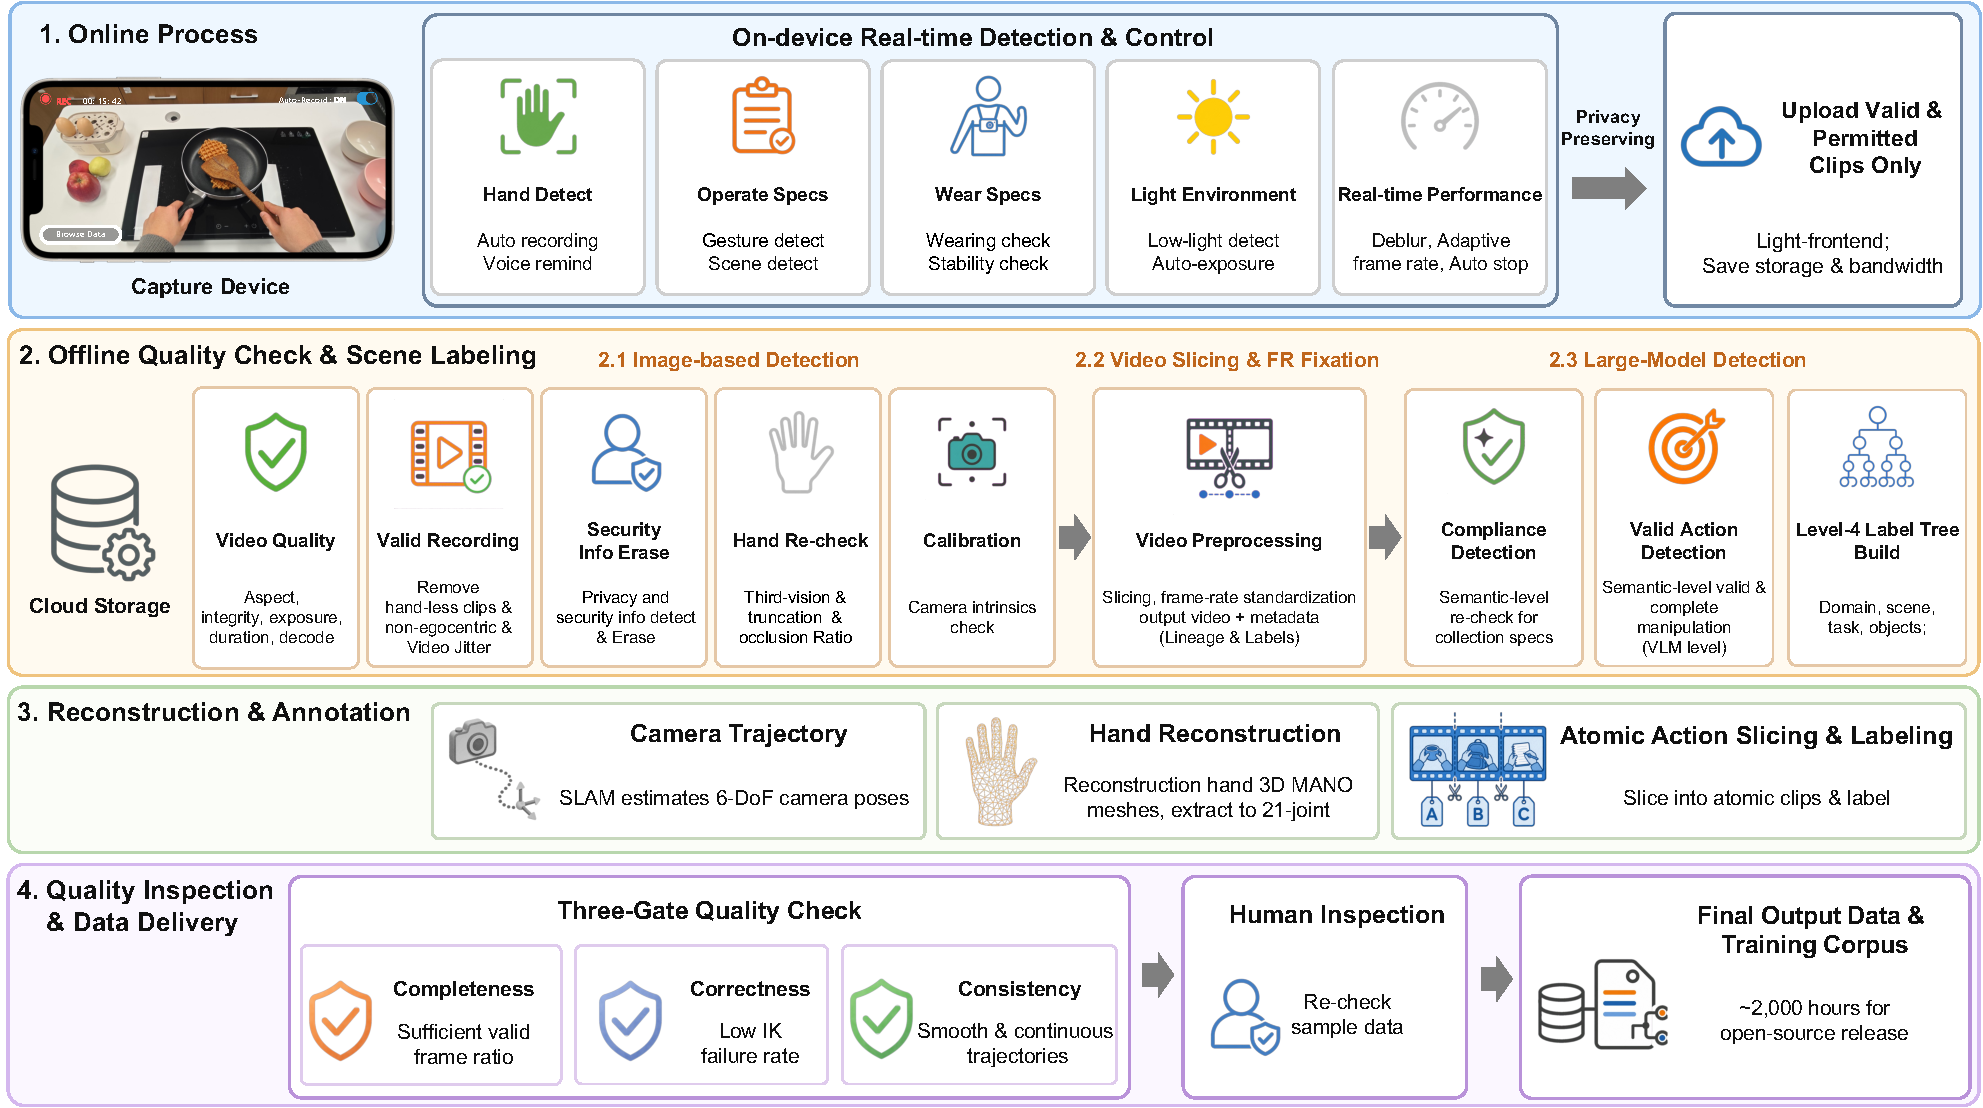
\includegraphics[width=\linewidth]{figures/fig2-data-pipline.pdf}
    \captionof{figure}{\textbf{Open-AoE data processing pipeline.} Starting from edge-side on-device detection and control, raw egocentric videos pass through offline quality checking and scene labeling (image-based detection, video slicing, and large-model detection), followed by pose reconstruction, atomic-action annotation, and three-gate quality inspection to produce an anonymized training corpus. The released subset contains approximately 2,000 hours of egocentric manipulation video captured with consumer smartphones, together with English annotations, MANO hand poses, and camera trajectories.}
    \label{fig:data-pipeline}
\end{center}

As shown in Figure~\ref{fig:data-pipeline}, the pipeline comprises an online capture stage and an offline processing stage.
It proceeds through four stages, namely edge-side online detection, offline quality checking with scene labeling, reconstruction and annotation, and quality inspection with data delivery, and finally produces the anonymized training corpus.

\subsection{Edge-side Online Detection}

On the capture device, lightweight on-device vision models gate recording in real time and govern capture quality, so that only clips containing meaningful hand-object interaction are retained~\cite{aoe2026}.
A hand-visibility check starts recording automatically once hands appear and stops it when they leave the frame, and prompts the user by voice to readjust whenever a hand reaches the image border or becomes truncated, which keeps the manipulating subject fully visible.
Operating and wearing compliance are monitored at the same time. The operating-spec check combines gesture detection with scene detection to flag non-standard actions and non-compliant capture scenes, while the wearing-spec check performs both a wearing check and a stability check to correct improper wearing poses and unstable views; either kind of issue is reported to the user through real-time voice feedback.
The device also adapts to the lighting environment by turning on a constant fill light together with global auto-exposure under dim light, and it sustains real-time performance through a fixed focal length, motion stabilization, deblurring, and an adaptive frame rate, halting recording when storage becomes insufficient or the device overheats.
This lightweight front-end design protects privacy at the source, saves storage and bandwidth, and uploads only valid and permitted clips to the cloud for offline processing.

\subsection{Offline Quality Check \& Scene Labeling}

\subsubsection{Image-based Detection}

The first gate operates on sampled frames without deep models, relying on image-analysis algorithms and lightweight detectors.
For video quality, a bank of rule-based detectors runs in parallel to flag the common defects that make recordings unusable, covering aspect ratio and rotation, file-header and stream integrity, pure-black or over- and under-exposed frames, insufficient duration, and decoding integrity, so that clearly corrupted videos are discarded early.
A valid-recording check then removes clips without visible hands, non-egocentric recordings such as fixed-mount or third-person side views, and segments with severe camera jitter, leaving only valid first-person manipulation.
Security-information erasure detects faces and other sensitive content and masks (pixelates) them in the frames, and it further replaces the personally identifiable information in the metadata, including the collector's name and contact, with anonymized identifiers while rewriting the corresponding fields and directory names; the mapping is stored in full and supports incremental reuse, so the process can be safely re-run and the anonymization reversed when authorized.
A hand re-check then verifies that both hands remain clearly visible by screening for residual third-person views, hand truncation, and an excessive occlusion ratio; a defect is confirmed only when it persists across several consecutive frames, which suppresses single-frame noise.
Calibration finally validates the camera intrinsics for completeness and validity, since reliable calibration is a prerequisite for later pose reconstruction.

\subsubsection{Video Slicing and Frame-Rate Fixation}

After image-based detection, the video is split along contiguous qualified and unqualified spans and its frame rate is fixed, so that a long recording becomes several semantically independent segments (termed \emph{Parts}), with qualified segments that are too short flagged separately.
Each Part stays linked to its source video through a unified process-tag file that records the data lineage from the raw video to each Part and accumulates multi-level labels as the pipeline advances, establishing a data contract that holds throughout the pipeline.

\subsubsection{Large-Model Detection}

Qualified Parts then move to the large-model stage, where the vision-language model Qwen3.7-Plus performs higher-level semantic detection and scene labeling.
Compliance detection re-checks at the semantic level whether a segment follows the collection specifications and identifies violations that are difficult to detect at the image level, while valid-action detection judges whether the action is valid and forms a complete, purposeful manipulation, complementing the earlier image-level screening.
The same model then constructs a four-level label tree under a closed-set design, assigning a representative frame exactly one domain, one scene, and one task from predefined sets together with the salient objects it contains, after which these outputs are standardized into unified identifiers and accumulated over the domain, scene, task, and object dimensions to form a hierarchical label system.

\subsection{Reconstruction \& Annotation}

Each qualified Part enters reconstruction, where camera-trajectory estimation, hand reconstruction, and atomic-action annotation are produced together.
Camera poses are recovered by DROID-W~\cite{droidw2026}, whose robust kernels are re-tuned for handheld and wearable capture to keep the 6-DoF trajectory stable under severe camera shake and torso-motion interference.
Hand reconstruction starts from a two-hand detector trained on large-scale egocentric data collected through AoE, which supplies per-frame bounding boxes, links detections across frames, and fills in missing or occluded hands; building on these boxes, HaWoR~\cite{hawor2025} recovers 3D MANO~\cite{mano2017} meshes that are metric-scale aligned through SLAM and brought into world coordinates, with sliding-window optimization enforcing temporal consistency.
A global bundle adjustment over the HaWoR reconstruction and the dynamic-object masks from DROID-W then optimizes the hand meshes and the camera trajectory jointly in a single world coordinate frame, removing the scale drift and coordinate mismatch that arise across segment-wise reconstructions.
From the recovered meshes, 21-joint hand keypoints are extracted, and each video is finally segmented into semantically coherent atomic clips labeled in English, with a human-in-the-loop review correcting model hallucinations.

\subsection{Quality Inspection \& Data Delivery}

The reconstructed and annotated Parts pass a three-gate quality inspection before archiving, from which about 2{,}000 hours are curated from the full data pool for open-source release.
The completeness gate retains Parts whose hand-reconstruction valid-frame ratio is high enough for reliable pose annotation; the correctness gate retains those whose inverse-kinematics failure rate stays low when retargeting to the 28-DoF joint space, which preserves downstream usability; and the consistency gate retains Parts with smooth, continuous camera trajectories free of abrupt jumps between adjacent frames.
Finally, a randomly sampled subset undergoes human inspection to confirm annotation accuracy and to remove edge cases such as severe occlusion or extreme lighting, yielding the anonymized training corpus that constitutes the final output.

\subsection{Data Distribution Analysis}
\label{sec:data-distribution}

Figure~\ref{fig:data-distribution} summarizes the diversity observed in a randomly sampled 100-hour subset of the Open-AoE release. All panels use this same sampling scope, including semantic content, collection context, anonymous contributor coverage, consumer-phone models, and horizontal field of view (FOV).
Wedge area, bar height, and word size encode relative prevalence or frequency rather than absolute duration.

\begin{figure*}[t]
    \centering
    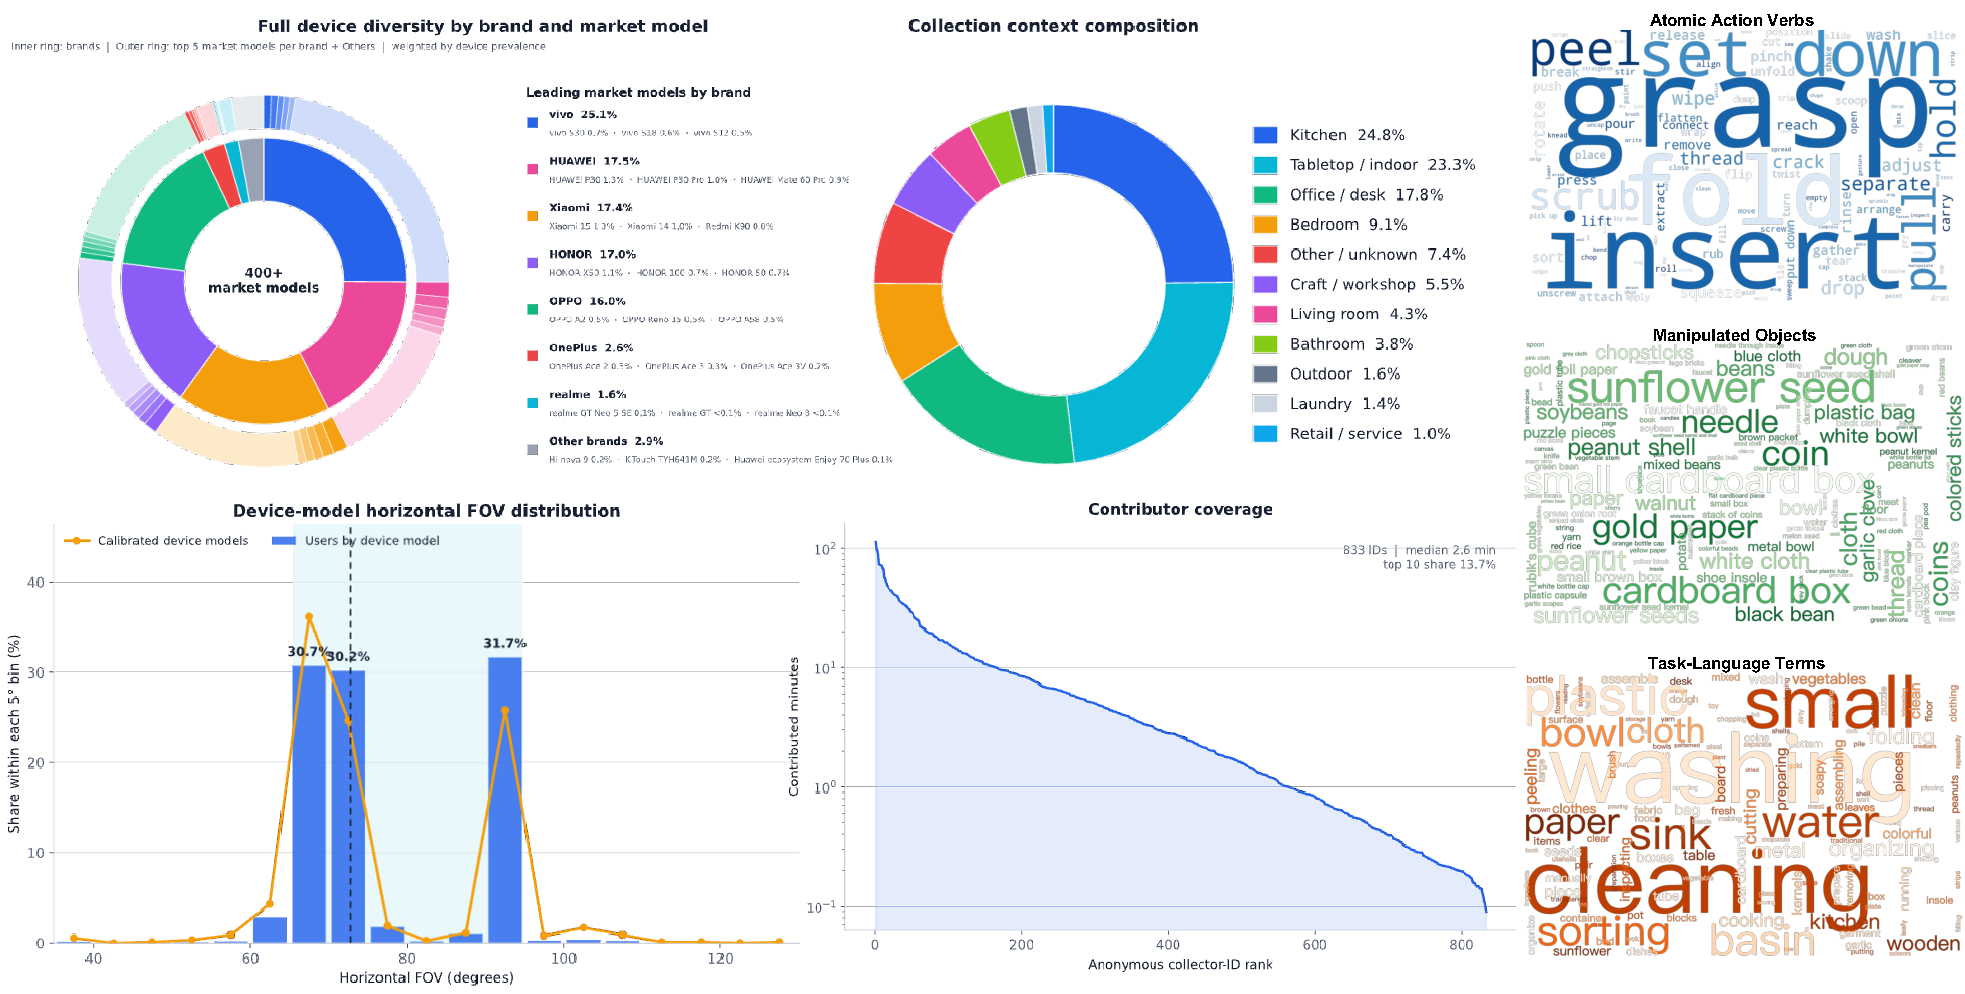
\includegraphics[width=\linewidth]{figures/fig-data-distribution.pdf}
    \caption{\textbf{Open-AoE collection, sensor, and semantic diversity in a random 100-hour sample.} The nested donut summarizes the consumer-phone brand and market-model composition, and the lower-left panel shows the horizontal-FOV distribution. The center panels report collection-context composition and anonymous collector-ID coverage, while the word clouds summarize atomic-action verbs, manipulated objects, and task-language terms. All panels use the same randomly sampled 100-hour subset; wedge area, bar height, and word size encode relative prevalence or frequency.}
    \label{fig:data-distribution}
\end{figure*}

\paragraph{Broad scenes, actions, and interaction objects.}
The updated 100-hour audit used in Section~\ref{sec:dataset-analysis} contains \textbf{32{,}407 distinct natural-language action descriptions}, \textbf{175 action verbs}, \textbf{8{,}030 object strings}, and \textbf{135 scene labels}.
As reported in Figure~\ref{fig:temporal_semantic}, the updated temporal annotations achieve \textbf{99.99\% temporal coverage}, with a mean segment duration of \textbf{9.64~s} and an annotation density of \textbf{13.97 segments per minute}.
Temporal coverage is computed from the union of annotated time spans, whereas mean duration and density are computed over annotation records; these quantities should therefore not be multiplied as if the annotations formed a strictly non-overlapping partition. These values supersede the interval and vocabulary counts from an earlier preprocessing snapshot.
These distributions cover reusable manipulation primitives together with a long tail of foods, tools, containers, craft materials, garments, and household objects.
Kitchens, tabletop or indoor settings, offices or desks, and bedrooms account for 24.8\%, 23.3\%, 17.8\%, and 9.1\%, respectively, while the remainder spans living rooms, workshops, bathrooms, outdoor areas, laundry spaces, and retail or service settings.
The joint diversity of scene, action, and interaction object provides a substrate for compositional generalization.

\paragraph{Distributed contributor coverage.}
The same 100-hour sample exhibits a long-tailed distribution across anonymous collector IDs. The median contribution is 2.6 minutes per ID, and the ten largest contributors together account for only 13.7\% of sampled duration.
This long-tailed coverage indicates that the sample is not dominated by a small group of collectors, preserving broader variation in manipulation habits, hand appearance, and recording environments.

\paragraph{A broad consumer-camera domain.}
The random 100-hour sample covers \textbf{400+ consumer-smartphone market models}. The nested donut groups brands in the inner ring and exposes leading models plus the aggregated model tail in the outer ring.
To our knowledge, this is the broadest reported consumer-phone device coverage for an egocentric manipulation dataset.
Restricting device statistics to the same random sample makes the model, semantic, context, and contributor distributions directly comparable under one evaluation scope.
The resulting breadth provides substantial consumer-camera domain diversity within the sampled subset.
Device identity is also a practical proxy for the underlying camera stack, including the lens, sensor, image-signal processor, resolution mode, exposure pipeline, and capture firmware.
Compared with a single-headset collection, Open-AoE therefore introduces naturally occurring camera-domain variation at capture time.

\paragraph{Optical diversity for robust visual transfer.}
Within the random 100-hour sample, the user-weighted horizontal-FOV distribution is multimodal: its three dominant 5-degree bins account for \textbf{30.7\%, 30.2\%, and 31.7\%}, concentrated around $65^{\circ}$--$75^{\circ}$ and $90^{\circ}$--$95^{\circ}$.
The multimodal profile reflects recurring camera and lens configurations rather than one optical system.
A downstream visual policy must recover hand-object geometry and motion across different projections, crops, distortions, and imaging pipelines.
This variation provides a form of natural sensor-domain randomization that may improve robustness when transferring to unseen cameras, deployment rigs, and robot viewpoints.

\textbf{Takeaway.} Open-AoE is differentiated not only by scale, but by diversity at three coupled levels: what people manipulate, where and how they act, and the consumer-camera domain through which every interaction is observed.
Together, these properties create a stronger basis for visually robust, cross-domain manipulation learning.

\textit{Scope and claim boundary.} Every distribution reported in this subsection is computed from the same random 100-hour sample. The downstream benefit of camera-domain diversity remains a training hypothesis that should be validated through controlled ablations.
